% Prosecutorial Policy Analysis — Funder Presentation
% Dvir Yogev · UC Berkeley School of Law
% February 2026

\documentclass[aspectratio=169, 11pt]{beamer}

% ---------- Theme & Colors ----------
\usetheme{metropolis}
\usepackage{appendixnumberbeamer}
\usepackage{booktabs}
\usepackage{multirow}
\usepackage{graphicx}
\usepackage{xcolor}
\usepackage{tikz}
\usepackage{tabularx}
\usepackage{array}
\usepackage{ragged2e}
\usepackage{fontspec}

% Custom colors
\definecolor{berkeleyblue}{HTML}{003262}
\definecolor{californiagold}{HTML}{FDB515}
\definecolor{foundersrock}{HTML}{3B7EA1}
\definecolor{medalistgreen}{HTML}{00B0B9}
\definecolor{alertred}{HTML}{ED4E33}
\definecolor{lightgray}{HTML}{F0F0F0}

\setbeamercolor{frametitle}{bg=berkeleyblue, fg=white}
\setbeamercolor{title}{fg=berkeleyblue}
\setbeamercolor{progress bar}{fg=californiagold}
\setbeamercolor{alerted text}{fg=alertred}
\setbeamercolor{block title}{bg=berkeleyblue, fg=white}
\setbeamercolor{block body}{bg=lightgray}
\setbeamercolor{block title alerted}{bg=alertred, fg=white}
\setbeamercolor{block body alerted}{bg=lightgray}
\setbeamercolor{block title example}{bg=medalistgreen, fg=white}
\setbeamercolor{block body example}{bg=lightgray}

\setbeamerfont{title}{size=\Large, series=\bfseries}
\setbeamerfont{frametitle}{size=\large}

% Shrink table fonts
\newcommand{\tablefont}{\fontsize{7.5}{9.5}\selectfont}
\newcommand{\smalltable}{\fontsize{6.5}{8.5}\selectfont}

% ---------- Metadata ----------
\title{Prosecutorial Policy Analysis}
\subtitle{AI-Powered Measurement of Criminal Justice Reform in California}
\author{Dvir Yogev}
\institute{Center for Law \& Justice, UC Berkeley School of Law}
\date{February 2026}

% ================================================================
\begin{document}

% ---------- TITLE ----------
\maketitle

% ---------- SLIDE: The Research Problem ----------
\begin{frame}{The Measurement Gap}
\begin{columns}[T]
\begin{column}{0.55\textwidth}
District Attorneys are among the \textbf{most powerful actors} in the criminal justice system, yet we lack systematic measurement of:
\begin{itemize}
    \item How their policies \textbf{vary across jurisdictions}
    \item How policies \textbf{change over time}
    \item Whether stated policy intent \textbf{affects outcomes}
\end{itemize}
\vspace{6pt}
Existing research relies on case outcomes or campaign rhetoric---neither captures the \emph{stated policy intent} that guides line prosecutors daily.
\end{column}
\begin{column}{0.42\textwidth}
\begin{alertblock}{What's Missing}
No systematic, comparable measurement of internal DA policy documents exists \textbf{anywhere}.
\end{alertblock}
\vspace{6pt}
\begin{exampleblock}{What We Built}
The first large-scale, AI-coded dataset of internal DA policy documents---infrastructure for causal inference about prosecutorial ideology.
\end{exampleblock}
\end{column}
\end{columns}
\end{frame}

% ---------- SLIDE: Data Source ----------
\begin{frame}{Data: ACLU NorCal Public Records Archive}
\begin{columns}[T]
\begin{column}{0.55\textwidth}
\textbf{2,665 internal DA policy documents} obtained by ACLU of Northern California via the California Racial Justice Act.
\begin{itemize}
    \item \textbf{41 of 58} California counties represented
    \item Charging directives, sentencing memos, diversion protocols, racial equity initiatives, bail reform orders
    \item Documents span 2015--2024
\end{itemize}
\vspace{4pt}
These are \emph{internal operating documents}---not press releases or campaign materials. They reveal what prosecutors actually tell their staff to do.
\end{column}
\begin{column}{0.42\textwidth}
\begin{block}{Why This Is Rare}
Internal policy memos are almost never publicly available. The ACLU's PRA effort created a \textbf{unique research opportunity} that may not persist indefinitely.
\end{block}
\end{column}
\end{columns}
\end{frame}

% ---------- SLIDE: The Pipeline ----------
\begin{frame}{What We Built: Research Pipeline}
\begin{center}
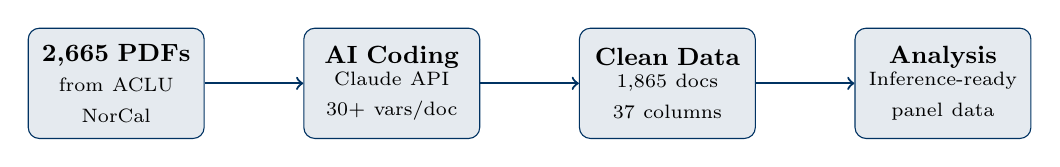
\begin{tikzpicture}[
    box/.style={rectangle, draw=berkeleyblue, fill=berkeleyblue!10, rounded corners, minimum width=2.2cm, minimum height=1.4cm, text width=2cm, align=center, font=\small},
    arrow/.style={->, thick, berkeleyblue}
]
\node[box] (a) at (0,0)   {\textbf{2,665 PDFs}\\\scriptsize from ACLU NorCal};
\node[box] (b) at (3.5,0) {\textbf{AI Coding}\\\scriptsize Claude API\\\scriptsize 30+ vars/doc};
\node[box] (c) at (7,0)   {\textbf{Clean Data}\\\scriptsize 1,865 docs\\\scriptsize 37 columns};
\node[box] (d) at (10.5,0){\textbf{Analysis}\\\scriptsize Inference-ready\\\scriptsize panel data};
\draw[arrow] (a) -- (b);
\draw[arrow] (b) -- (c);
\draw[arrow] (c) -- (d);
\end{tikzpicture}
\end{center}
\vspace{-2pt}
{\tablefont
\begin{tabularx}{\textwidth}{lX}
\toprule
\textbf{Dimension Coded} & \textbf{What's Measured} \\
\midrule
Ideological Orientation & 7-point scale: clearly progressive $\to$ clearly traditional \\
Extensive Margin & Impact on \emph{who enters} the system (charging, diversion) \\
Intensive Margin & Impact on \emph{how severely} people are treated (sentencing) \\
Specific Policies & Diversion, bail reform, enhancements, three strikes, racial justice \\
Administrative Context & New policy vs.\ continuation, DA administration \\
\bottomrule
\end{tabularx}}
\vspace{2pt}
\begin{center}\scriptsize Total API cost: \textasciitilde\$80 \quad$\cdot$\quad Processing time: \textasciitilde 2 hours\end{center}
\end{frame}

% ---------- SLIDE: Face Validity ----------
\begin{frame}{Face Validity: The Pipeline Recovers Known Patterns}
{\small\color{gray} These findings build confidence that the AI coding measures real variation.}
\vspace{4pt}
\begin{columns}[T]
\begin{column}{0.48\textwidth}
\begin{block}{Gasc\'on Transformation}
LA County ideology score \textbf{tripled} under Gasc\'on\\
Cohen's $d = 0.75$, $p < 0.001$
\end{block}
\vspace{4pt}
\begin{block}{Geographic Clustering}
\begin{itemize}\setlength\itemsep{1pt}
    \item \textcolor{medalistgreen}{\textbf{Progressive:}} Sacramento $+78\%$, Yolo $+56\%$, San Diego $+50\%$
    \item \textcolor{alertred}{\textbf{Traditional:}} Stanislaus $-34\%$, Placer $-21\%$
    \item Bay Area variation: Santa Clara $+0.84$ vs Alameda $-0.15$
\end{itemize}
\end{block}
\end{column}
\begin{column}{0.48\textwidth}
\begin{block}{2020 Racial Justice Surge}
Racial justice emphasis jumped \textbf{+30pp} in one year (12\% $\to$ 42\%), tracking the post-George Floyd moment precisely.
\vspace{3pt}
Documents with high racial justice emphasis are \textbf{4.6$\times$} more likely to be progressive ($\chi^2 = 421$, $p < 0.001$).
\end{block}
\vspace{4pt}
\begin{exampleblock}{Why This Matters}
Pipeline confirms patterns any expert would expect---evidence of validity, not artifact.
\end{exampleblock}
\end{column}
\end{columns}
\end{frame}

% ---------- SLIDE: Descriptive Analysis ----------
\begin{frame}{Descriptive Analysis: Theory-Grounded Patterns}
\begin{columns}[T]
\begin{column}{0.48\textwidth}
\begin{block}{Extensive $>$ Intensive Margin}
Recent reforms disproportionately emphasize \textbf{who enters} the system (\textbf{33.9\%} extensive lenient) over \textbf{how severely} people are treated (\textbf{22.6\%} intensive lenient).
\vspace{4pt}
{\small\color{gray} Political economy logic: diversion/declination less visible to voters than sentencing leniency---safer reforms for DAs facing reelection.}
\end{block}
\end{column}
\begin{column}{0.48\textwidth}
\begin{block}{Close Elections $\to$ Progressive Policy}
Elections with margins $\leq$15pp produce \textbf{+31.2pp} more progressive policies ($p = 0.010$).
\vspace{4pt}
Continuous: $r = -0.50$ between margin and ideology ($p = 0.009$).
\vspace{4pt}
{\small\color{gray} Provides credible first stage for instrumental variables designs.}
\end{block}
\end{column}
\end{columns}
\vspace{8pt}
\begin{alertblock}{}
\textbf{Novel contributions:} The extensive-over-intensive pattern has not been documented at this scale. The election-ideology link provides the first stage for causal designs.
\end{alertblock}
\end{frame}

% ---------- SLIDE: Policy Shocks ----------
\begin{frame}{In the Service of Causal Inference: Policy Shocks}
{\small The pipeline detects sharp policy transitions---the quasi-experimental variation causal designs require.}
\vspace{6pt}
\begin{columns}[T]
\begin{column}{0.48\textwidth}
\begin{block}{Disruptions Detected}
\begin{itemize}\setlength\itemsep{2pt}
    \item \textbf{9} significant policy disruptions (2020--23)
    \item SF 2020 (Boudin): highest score (0.572)
    \item \textbf{347} novel reform adoptions tracked
\end{itemize}
\end{block}
\vspace{4pt}
\begin{block}{Progressive Surge (2019--2022)}
\begin{itemize}\setlength\itemsep{2pt}
    \item Progressive docs: 18\% $\to$ 40\% $\to$ 56\%
    \item Linear trend: $+0.062$/yr ($p = 0.003$, $R^2 = 0.52$)
    \item Gradual trend + sharp county disruptions
\end{itemize}
\end{block}
\end{column}
\begin{column}{0.48\textwidth}
\begin{exampleblock}{Why Funders Should Care}
\begin{itemize}\setlength\itemsep{3pt}
    \item Each disruption $=$ potential ``natural experiment''
    \item Staggered adoption $\to$ modern DiD/event study designs
    \item Combined with outcome data $\to$ credible causal estimates
\end{itemize}
\end{exampleblock}
\end{column}
\end{columns}
\end{frame}

% ---------- SLIDE: Jail Data Pilot ----------
\begin{frame}{Jail Data Pilot: First Steps Toward Causal Evidence}
{\small Linked AI-coded policy scores to \textbf{Vera Institute Incarceration Trends} (245,840 quarterly obs., all US counties).}
\vspace{4pt}
{\tablefont
\begin{tabularx}{\textwidth}{lllX}
\toprule
\textbf{Finding} & \textbf{Estimate} & \textbf{Significance} & \textbf{Survives Controls?} \\
\midrule
Ideology $\leftrightarrow$ Jail Pop Rate & $r = -0.222$ & $p = 0.009$ & \textcolor{medalistgreen}{\textbf{Yes}} (year-demeaned) \\
Ideology $\leftrightarrow$ Jail Admissions & $r = -0.221$ & $p = 0.009$ & \textcolor{medalistgreen}{\textbf{Yes}} (year-demeaned) \\
Progressive vs Traditional & $-68.5$/100k & $d = -0.81$ & \textcolor{medalistgreen}{\textbf{Yes}} \\
LA Pretrial (Gasc\'on DiD) & $-32.1$/100k & Pre-trend $p = 0.90$ & \textcolor{medalistgreen}{\textbf{Cleanest}} \\
\bottomrule
\end{tabularx}}
\vspace{4pt}
\begin{columns}[T]
\begin{column}{0.48\textwidth}
\begin{exampleblock}{What Holds Up}
{\small Associations \textbf{survive year controls}. Pretrial detention shows cleanest causal signal (pre-trend $p = 0.90$).}
\end{exampleblock}
\end{column}
\begin{column}{0.48\textwidth}
\begin{alertblock}{What the Pilot Exposes}
{\small Naive pre/post \textbf{confounded by COVID}. Parallel trends violated ($p = 0.021$). TWFE non-significant ($N = 137$).}
\end{alertblock}
\end{column}
\end{columns}
\end{frame}

% ---------- SLIDE: What This Can Test ----------
\begin{frame}{What This Infrastructure Can Test}
{\small Each row is a testable causal question---the policy variation already exists in our data.}
\vspace{4pt}
{\smalltable
\begin{tabularx}{\textwidth}{p{3.2cm}Xp{4.2cm}}
\toprule
\textbf{DA Policy (Coded)} & \textbf{Measurable Outcome} & \textbf{Data Required} \\
\midrule
Bail/pretrial reform & Pretrial detention, FTA, pretrial crime & Vera (done); CA DOJ; CJARS \\
Diversion programs & Case dismissals, recidivism (1--3 yr) & UniCourt; CJARS recidivism \\
``Decline to prosecute'' memos & Filing rates: drugs, property, QOL & CA DOJ OpenJustice (free) \\
Enhancement/3-strikes reform & Sentence lengths, enhancement filings & CA Sentencing Comm.; CJARS \\
Racial equity directives & B/W disparities: charging, sentencing & CA DOJ by-race; CJARS \\
Extensive margin (who enters system) & System contact per capita; jail admissions & CA DOJ filings; Vera (done) \\
\bottomrule
\end{tabularx}}
\vspace{4pt}
\begin{block}{}
\textbf{The policy variation exists.} What's needed: outcome linkage (Extension 2) and geographic scale (Extension 1) to power DiD, RDD, event study, and synthetic control designs.
\end{block}
\end{frame}

% ---------- SLIDE: Extension 1 ----------
\begin{frame}{Extension 1: Expanding Policy Coverage}
\begin{columns}[T]
\begin{column}{0.48\textwidth}
\begin{block}{Within California}
\begin{itemize}\setlength\itemsep{2pt}
    \item Complete remaining \textbf{17 counties} via PRA
    \item \textbf{Pre-2015 historical} documents for longer pre-periods
    \item \textbf{200-doc human validation} for publication credibility
\end{itemize}
\end{block}
\end{column}
\begin{column}{0.48\textwidth}
\begin{block}{100 Largest DA Offices Nationwide}
\begin{itemize}\setlength\itemsep{2pt}
    \item \textasciitilde 65\% of US population covered
    \item \textbf{30--50 close elections} for RDD (vs \textasciitilde 5 in CA)
    \item Tests external validity across \textbf{different legal cultures}
\end{itemize}
\end{block}
\end{column}
\end{columns}
\vspace{6pt}
{\tablefont
\begin{tabularx}{\textwidth}{p{3.8cm}lXlr}
\toprule
\textbf{Scope} & \textbf{Scale} & \textbf{Enables} & \textbf{Time} & \textbf{Cost} \\
\midrule
Complete CA + historical & \textasciitilde 500 docs & Full panel; longer pre-periods & 4--6 mo & \textasciitilde\$25--35k \\
100 largest US DA offices & 5--10k docs & Powered RDD; national benchmarking & 12--18 mo & \textasciitilde\$100--150k \\
Human validation (200 docs) & 200 dual-coded & IRR; publication credibility & 3 mo & \textasciitilde\$20k \\
\bottomrule
\end{tabularx}}
\end{frame}

% ---------- SLIDE: Extension 2 ----------
\begin{frame}{Extension 2: Merging with Outcome Data}
\begin{columns}[T]
\begin{column}{0.48\textwidth}
\begin{block}{Administrative Data (Available Now)}
{\tablefont
\begin{tabularx}{\columnwidth}{lX}
\toprule
\textbf{Source} & \textbf{Records} \\
\midrule
CA DOJ OpenJustice & County-year arrest, filing, incarceration \\
CA Sentencing Comm. & Enhancement filings, 3-strikes usage \\
Vera (done) & Quarterly jail pop by county \\
\bottomrule
\end{tabularx}}
\end{block}
\end{column}
\begin{column}{0.48\textwidth}
\begin{block}{Case-Level Data (Higher Return)}
{\tablefont
\begin{tabularx}{\columnwidth}{lX}
\toprule
\textbf{Source} & \textbf{Records} \\
\midrule
UniCourt / PACER & Case dispositions, plea bargains \\
CJARS & Arrest $\to$ parole, 24 states \\
\bottomrule
\end{tabularx}}
\end{block}
\end{column}
\end{columns}
\vspace{6pt}
\begin{exampleblock}{CJARS (Census Bureau + U.\ Michigan)}
Harmonized individual-level criminal justice records across 24 states. Tracks people from arrest through parole. Enables testing whether a progressive DA's diversion memo actually reduces the probability an arrested individual proceeds to prosecution. Accessible via FSRDC (3--12 month application).
\end{exampleblock}
\end{frame}

% ---------- SLIDE: Policymaker Value ----------
\begin{frame}{Value for Policymakers}
\begin{columns}[T]
\begin{column}{0.48\textwidth}
\begin{itemize}\setlength\itemsep{6pt}
    \item \textbf{DA accountability scorecards}---comparable measures of how each office's stated policies align with its goals
    \item \textbf{Rhetoric vs.\ practice}---does a ``decline low-level drugs'' memo actually reduce drug prosecutions?
\end{itemize}
\end{column}
\begin{column}{0.48\textwidth}
\begin{itemize}\setlength\itemsep{6pt}
    \item \textbf{Benchmarking tools}---a DA considering bail reform can see how similar policies performed elsewhere
    \item \textbf{Causal evidence on the progressive prosecutor model}---answering the central question: does it work?
\end{itemize}
\end{column}
\end{columns}
\vspace{8pt}
\begin{block}{Related Work}
Felix Owusu's AV-funded project exploits two specific internal DA memos for a causal design. Our contribution scales this logic: \textbf{systematic measurement across 41+ offices and 1,865 documents}, creating variation needed for average causal effects and heterogeneity analysis.
\end{block}
\end{frame}

% ---------- SLIDE: Funding ----------
\begin{frame}{Recommended Funding Package}
{\tablefont
\begin{tabularx}{\textwidth}{p{1.2cm}Xp{1.4cm}rX}
\toprule
\textbf{Phase} & \textbf{Components} & \textbf{Timeline} & \textbf{Budget} & \textbf{Deliverable}\\
\midrule
\textbf{1} & CA DOJ outcome linkage; complete CA panel; human validation & 6 mo & \$45--50k & First causal estimates (DiD/SC) with validated measurement \\
\addlinespace
\textbf{2} & 100 largest US DA offices; national election DB; CJARS application & 12--18 mo & \$100--150k & National DA ideology DB; powered RDD \\
\addlinespace
\textbf{3} & Case-level data (UniCourt/CJARS); stakeholder interviews & 6--12 mo & \$50--65k & Mechanism evidence: what changes in courtrooms \\
\bottomrule
\end{tabularx}}
\vspace{10pt}
\begin{center}
{\Large\textbf{\textcolor{berkeleyblue}{\$200--265k}} over 24--36 months}
\vspace{4pt}

{\small The infrastructure is built. The marginal cost of each extension is low---the pipeline, coding schema, and analysis framework are ready to scale.}
\end{center}
\end{frame}

% ---------- SLIDE: Why Now ----------
\begin{frame}{Why Fund This Now}
\begin{columns}[T]
\begin{column}{0.48\textwidth}
\begin{block}{Unique Advantages}
\begin{itemize}\setlength\itemsep{3pt}
    \item \textbf{Infrastructure is built}---pipeline, schema, analysis framework operational
    \item \textbf{Data window is closing}---ACLU PRA archive may not persist
    \item \textbf{No competitor}---no other systematic, AI-coded DA policy database exists
    \item \textbf{Pilot-tested}---demonstrated linkage to outcomes; identified the right methods
\end{itemize}
\end{block}
\end{column}
\begin{column}{0.48\textwidth}
\begin{block}{Policy Impact}
\begin{itemize}\setlength\itemsep{3pt}
    \item Answers the question \textbf{funders care about most}: do progressive reforms actually work?
    \item Enables \textbf{evidence-based evaluation} of DA accountability efforts
    \item Creates \textbf{benchmarking tools} for jurisdictions
    \item First \textbf{causal estimates} of prosecutorial policy effects
\end{itemize}
\end{block}
\end{column}
\end{columns}
\end{frame}

% ---------- SLIDE: CTA ----------
{
\setbeamercolor{background canvas}{bg=berkeleyblue}
\setbeamercolor{normal text}{fg=white}
\usebeamercolor[fg]{normal text}
\begin{frame}[plain]
\vfill
\begin{center}
{\LARGE\textbf{Let's Talk}}
\vspace{16pt}

{\normalsize The descriptive associations are real. The causal question is answerable.\\
The infrastructure is ready. We need your support to get there.}
\vspace{24pt}

{\normalsize\textbf{Dvir Yogev}}\\
{\small Post-Doctoral Researcher $\cdot$ UC Berkeley School of Law}\\
{\small\textcolor{californiagold}{dyo@berkeley.edu}}
\vspace{16pt}

{\scriptsize\textcolor{californiagold}{github.com/dyo2112/prosecutor-policies-causal-inference}}\\
{\scriptsize Full pilot report, figures, and replication code available in repository}
\end{center}
\vfill
\end{frame}
}

% ================================================================
% BACKUP SLIDES
% ================================================================
\appendix

{
\setbeamercolor{background canvas}{bg=berkeleyblue!90}
\setbeamercolor{normal text}{fg=white}
\usebeamercolor[fg]{normal text}
\begin{frame}[plain]
\vfill
\begin{center}
{\Large\textbf{Backup Slides}}
\end{center}
\vfill
\end{frame}
}

% ---------- BACKUP: Overcoming Limitations ----------
\begin{frame}[shrink=15]{Overcoming Pilot Limitations}
{\smalltable
\begin{tabularx}{\textwidth}{p{2.8cm}p{3.5cm}X}
\toprule
\textbf{Limitation} & \textbf{Root Cause} & \textbf{Solution} \\
\midrule
COVID confounds DiD & All CA counties declined in 2020 & Multi-state data diversifies; synthetic control matches on pre-treatment trajectories \\
\addlinespace
Parallel trends violated ($p = 0.021$) & LA converging pre-Gasc\'on & Longer pre-period (pre-2015 docs) + case-level data \\
\addlinespace
TWFE non-significant ($N = 137$) & Only 34 counties, 9 years & Extension 1 (national) increases $N$ and DA transitions \\
\addlinespace
Aggregate data too coarse & Cannot distinguish mechanisms & Extension 2 (UniCourt, CJARS): mechanism decomposition \\
\bottomrule
\end{tabularx}}
\end{frame}

% ---------- BACKUP: Causal Strategies ----------
\begin{frame}[shrink=15]{Causal Identification Strategies}
{\smalltable
\begin{tabularx}{\textwidth}{p{2.2cm}p{3.2cm}p{2.5cm}X}
\toprule
\textbf{Design} & \textbf{Current Status} & \textbf{What's Needed} & \textbf{Extension} \\
\midrule
RDD & \textasciitilde 5 close CA elections---underpowered & 30--50 close elections & Extension 1 (national) \\
\addlinespace
Stacked DiD & 9 disruptions; Vera outcomes only & Crime/sentencing outcomes + more transitions & Extensions 1 + 2 \\
\addlinespace
Synthetic Control & Gasc\'on pilot works; limited outcomes & Outcome data beyond jail pop & Extension 2 \\
\addlinespace
Event Study & Pre-period marginal (6 yrs) & Longer pre-period (pre-2015) & Extension 1 \\
\addlinespace
Instrumental Variables & Election margin $\to$ ideology ($r = -0.50$) & Outcome data for second stage & Extension 2 \\
\bottomrule
\end{tabularx}}
\end{frame}

% ---------- BACKUP: Extension 2 Detail ----------
\begin{frame}[shrink=15]{Extension 2 Detail: Outcome Data Sources}
{\smalltable
\begin{tabularx}{\textwidth}{p{2.5cm}Xp{1.4cm}rp{1.2cm}}
\toprule
\textbf{Source} & \textbf{Records} & \textbf{Timeline} & \textbf{Cost} & \textbf{Priority} \\
\midrule
CA DOJ OpenJustice & County-year arrest, filing, incarceration & Immediate & Free & High \\
\addlinespace
CA Sentencing Comm. & Enhancement filings, 3-strikes by county-year & 1--2 mo & Free & High \\
\addlinespace
Vera (done) & Quarterly jail pop and admissions & Done & Done & Done \\
\addlinespace
UniCourt / PACER & Individual case dispositions, plea bargains & 2--3 mo & \textasciitilde\$30--50k & Very high \\
\addlinespace
CJARS & Individual arrest $\to$ parole, 24 states & 3--12 mo & \textasciitilde\$5k & Highest \\
\bottomrule
\end{tabularx}}
\vspace{6pt}
\begin{exampleblock}{}
\textbf{Case-level data is the gold standard:} it links policy documents directly to line-prosecutor behavior. Are ``minimize enhancements'' memos actually reducing enhancement filings? UniCourt and CJARS can answer that.
\end{exampleblock}
\end{frame}

% ---------- BACKUP: Disruption Detection ----------
\begin{frame}{Policy Disruption Detection: Methodology}
{\tablefont
\begin{tabularx}{\textwidth}{lrX}
\toprule
\textbf{Signal} & \textbf{Weight} & \textbf{Method} \\
\midrule
Ideology Velocity & 30\% & Rate of ideology change vs.\ prior 2-year baseline \\
Novelty Index & 25\% & Proportion of first-time policy types \\
Topic Shift & 20\% & Jensen-Shannon divergence of topic distributions \\
Margin Reversal & 15\% & Flips in extensive/intensive leniency direction \\
DA Transition & 10\% & New administration detection \\
\bottomrule
\end{tabularx}}
\vspace{6pt}
\textbf{Top disruptions detected:}
\begin{enumerate}\setlength\itemsep{1pt}
    \item San Francisco 2020 (Boudin): 0.572
    \item LA County 2021 (Gasc\'on): 0.549
    \item Sacramento 2022: 0.412
\end{enumerate}
\end{frame}

% ---------- BACKUP: Anticipated Objections ----------
\begin{frame}{Anticipated Objections}
\begin{block}{``Policy documents $\neq$ practice. How do you know what's written actually happens?''}
{\small That's exactly why Extension 2 (outcome linkage) is Priority~1. We test whether ``diversion-positive'' memos predict more diversions. We also plan stakeholder interviews to validate. But note: even the stated-policy variation is \emph{itself} a novel descriptive contribution.}
\end{block}
\vspace{4pt}
\begin{block}{``You only have California. Isn't this just a Blue State story?''}
{\small That's the point of Extension 1. CA provides internal variation (progressive Bay Area vs.\ traditional Central Valley), but external validity requires national expansion. We target the 100 largest DA offices to include red/purple jurisdictions.}
\end{block}
\vspace{4pt}
\begin{block}{``AI coding isn't reliable enough for research.''}
{\small The face validity checks are strong ($d = 0.75$ Gasc\'on, geographic clustering). Phase~1 includes a 200-doc human validation study to establish gold-standard IRR. The \$80 cost and 2-hour runtime make iteration cheap.}
\end{block}
\end{frame}

\end{document}
